%============================ PLATAFORMA WEB (ENTREGA 2) ====================
\chapter{Plataforma web: interfaz, uso y comunicación}
\label{cap:plataforma}

Este capítulo documenta la plataforma de análisis y control de EILOR desde la
perspectiva de su uso: cómo se ingresa, qué opciones ofrece, cómo está construida
su interfaz y de qué manera se comunica con el dispositivo ESP32. La instancia de
referencia se encuentra publicada en \plataformaurl, servida a través del túnel de
Cloudflare descrito en el Capítulo~\ref{cap:cloudflare}.

\section{Acceso a la plataforma}
La plataforma se abre desde cualquier navegador moderno en la dirección pública
\plataformaurl{} o, en despliegues locales, en \code{http://localhost:3002}. Al
cargar, el \emph{dashboard} muestra de inmediato ---en modo de \emph{solo
lectura}--- el estado del ESP32, el modo activo, los contadores de dispositivos y
paquetes, el mapa de saturación espectral y el radar BLE, sin exigir credenciales.
Este acceso público de solo lectura permite observar el espectro sin poder emitir
comandos.

\subsection{Inicio de sesión}
Para habilitar las \emph{acciones de control} ---cambiar de modo, desplegar el
SoftAP, limpiar datos, listar o exportar registros--- se requiere iniciar sesión.
Al pulsar \emph{Iniciar Sesión} aparece el formulario de la Figura~\ref{fig:login},
que solicita la contraseña configurada en la variable de entorno
\code{EILOR\_PASSWORD}. Si la contraseña es correcta, el servidor emite un
\emph{token de sesión} (cadena hexadecimal de 48 caracteres, con vigencia de 24~h)
que el navegador conserva y adjunta en la cabecera \code{x-eilor-token} de cada
petición protegida. Una contraseña incorrecta devuelve \code{HTTP 401} y la sesión
no se habilita.

\begin{figure}[H]
\centering
\setlength{\fboxsep}{0pt}\setlength{\fboxrule}{0.4pt}%
\fcolorbox{gray!45}{white}{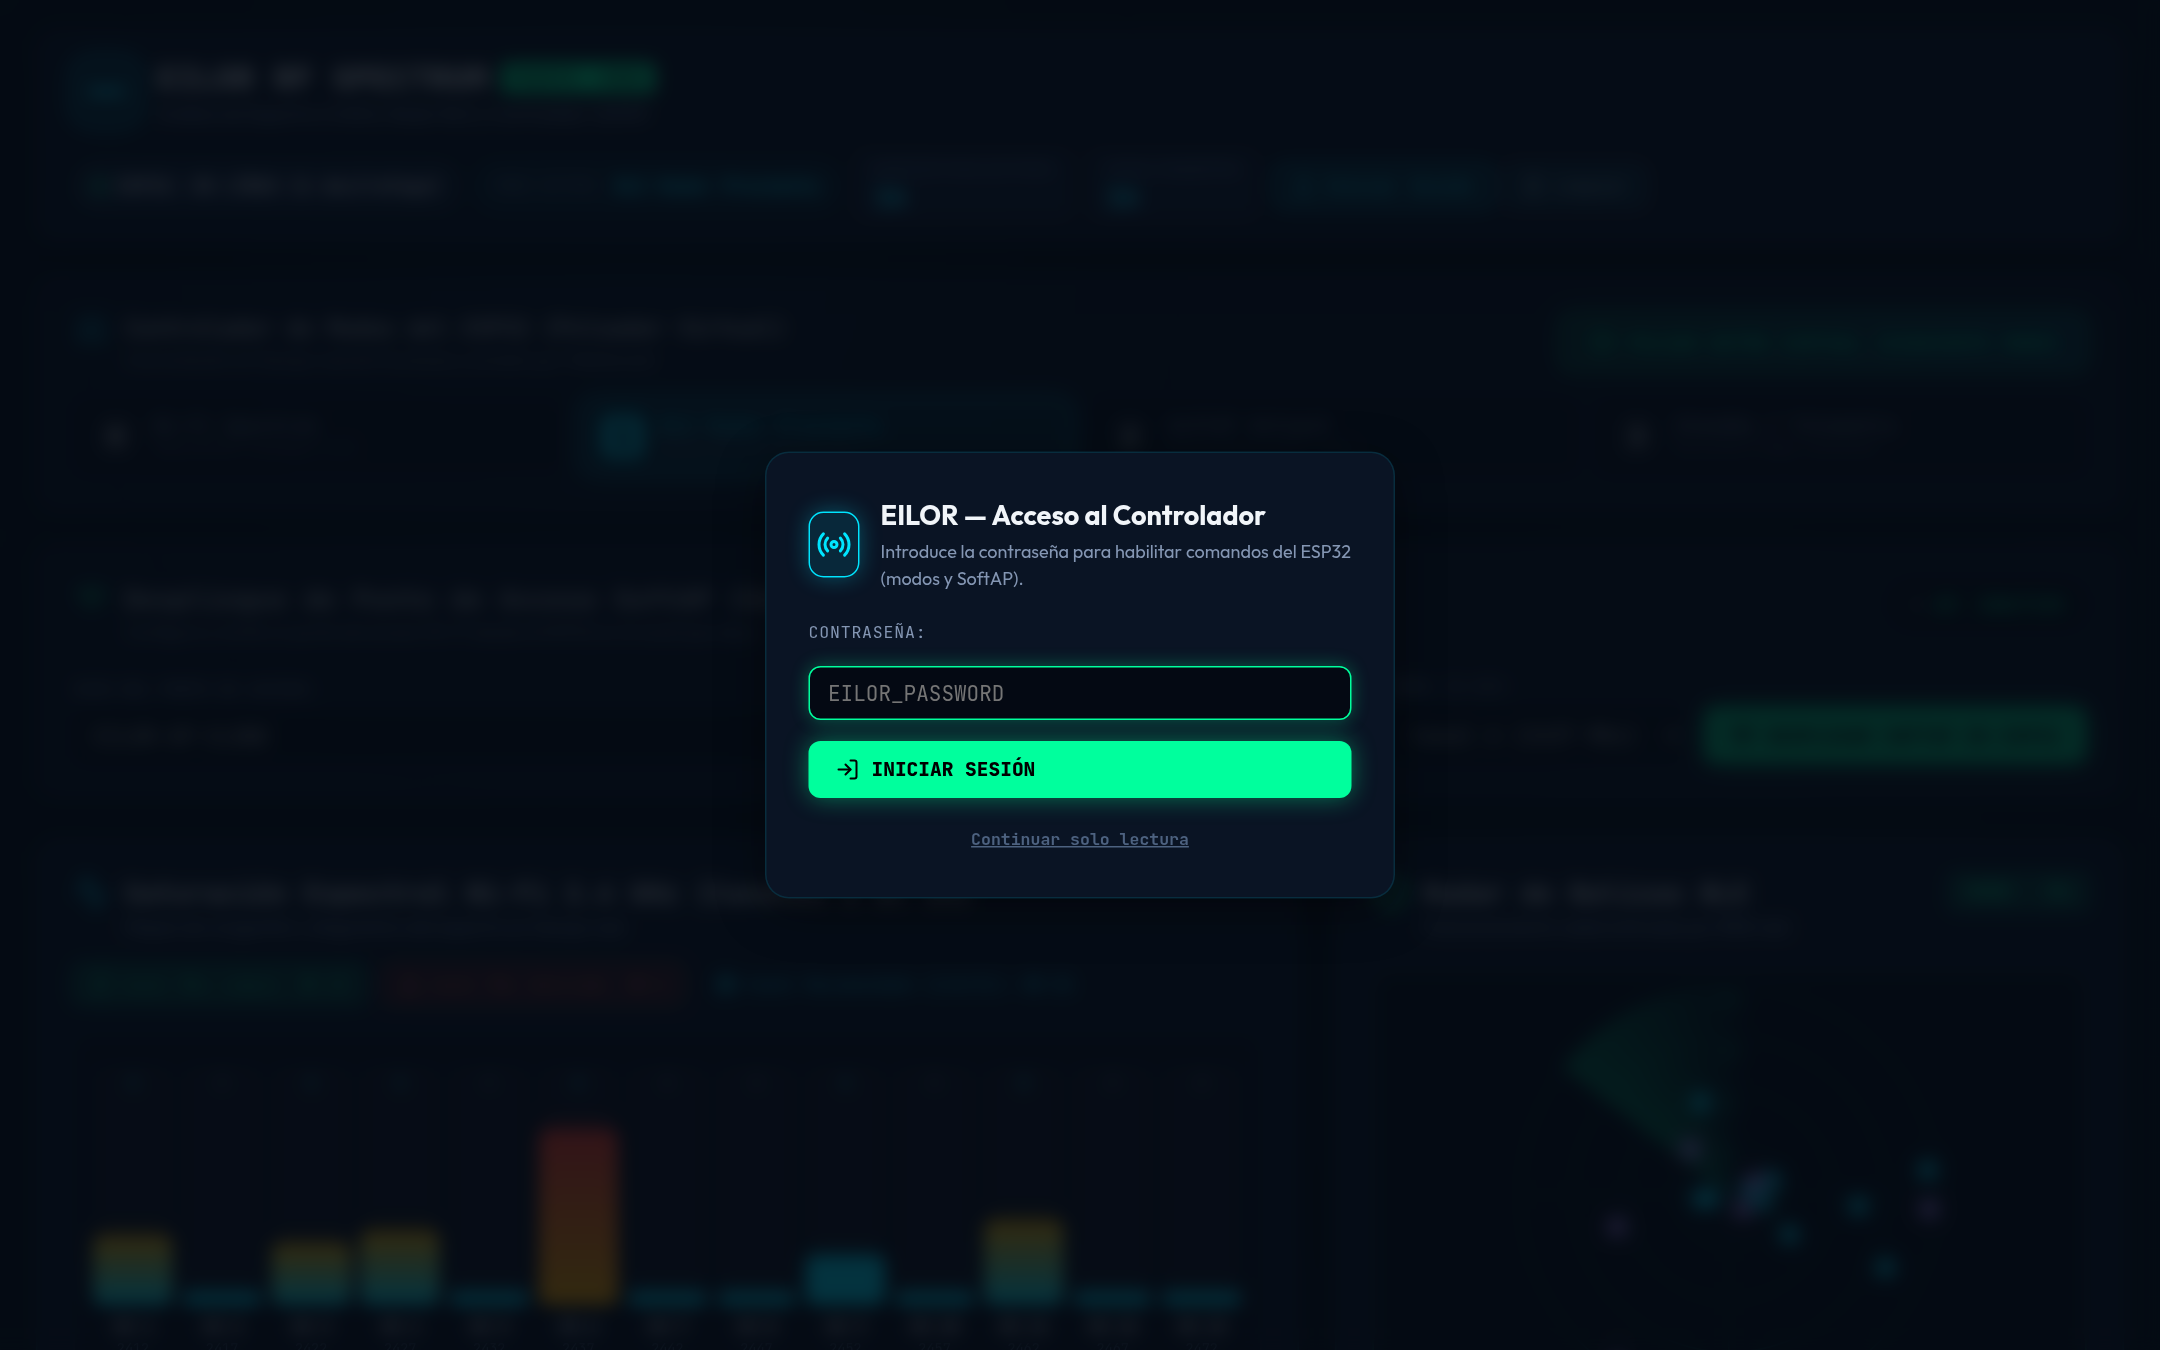
\includegraphics[width=0.78\linewidth]{figuras/cap-login}}
\caption{Formulario de inicio de sesión de la plataforma (habilita los comandos del ESP32).}
\label{fig:login}
\end{figure}

\section{Estructura y opciones de la interfaz}
El \emph{dashboard} organiza sus funciones en secciones apiladas verticalmente. La
Figura~\ref{fig:cabecera} muestra la cabecera de estado, con el indicador de
conexión del ESP32, el modo activo y los contadores globales, además de los botones
de sesión y de reinicio de datos.

\begin{figure}[H]
\centering
\setlength{\fboxsep}{0pt}\setlength{\fboxrule}{0.4pt}%
\fcolorbox{gray!45}{white}{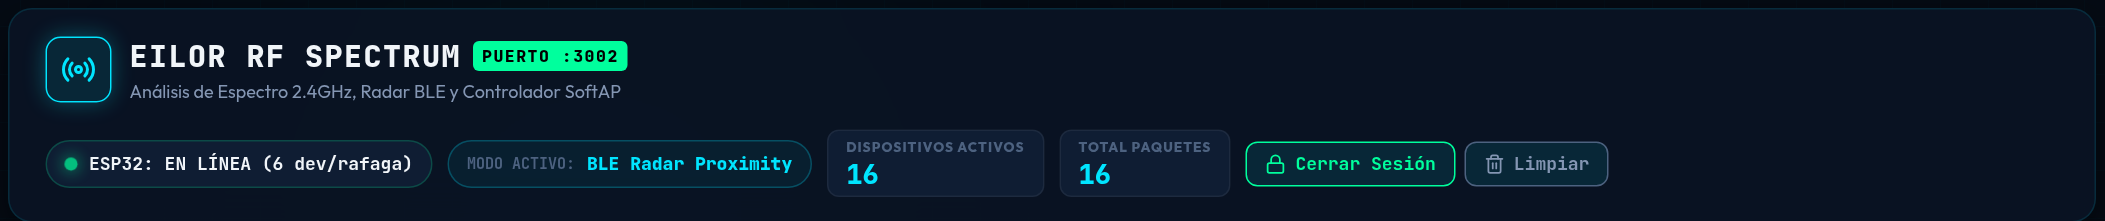
\includegraphics[width=0.98\linewidth]{figuras/cap-cabecera}}
\caption{Cabecera de estado: enlace del ESP32, modo activo y contadores de dispositivos y paquetes.}
\label{fig:cabecera}
\end{figure}

\subsection{Controlador de modos}
La sección \emph{Controlador de Modos} (Figura~\ref{fig:modos}) actúa como un
\emph{pulsador virtual}: replica en la web el botón físico del dispositivo. Permite
seleccionar directamente cualquiera de los cuatro modos ---(0)~Espectro Wi\nobreakdash-Fi,
(1)~Radar BLE, (2)~SoftAP con portal cautivo y (3)~Standby--- o avanzar al
siguiente. Cada cambio se emite por WebSocket y el ESP32 lo aplica en tiempo real.

\begin{figure}[H]
\centering
\setlength{\fboxsep}{0pt}\setlength{\fboxrule}{0.4pt}%
\fcolorbox{gray!45}{white}{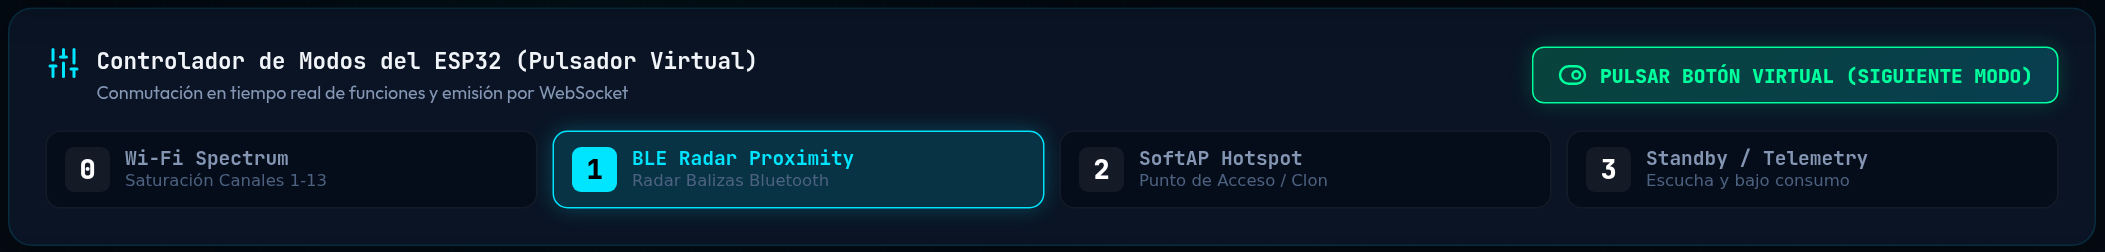
\includegraphics[width=0.98\linewidth]{figuras/cap-modos}}
\caption{Controlador de modos: conmutación remota de las cuatro funciones del ESP32.}
\label{fig:modos}
\end{figure}

\subsection{Despliegue del punto de acceso (SoftAP)}
En la sección \emph{Despliegue de Punto de Acceso} (Figura~\ref{fig:softap}) se
define el SSID y el canal (1--13) del punto de acceso propio y se pulsa
\emph{Desplegar SoftAP en ESP32}. El dispositivo pasa al modo~2, emite la red y
levanta el portal cautivo de registro. Esta funcionalidad está concebida
exclusivamente para redes propias, con un nombre identificable y aviso de registro,
conforme a las consideraciones éticas del Capítulo~\ref{cap:conclusiones}.

\begin{figure}[H]
\centering
\setlength{\fboxsep}{0pt}\setlength{\fboxrule}{0.4pt}%
\fcolorbox{gray!45}{white}{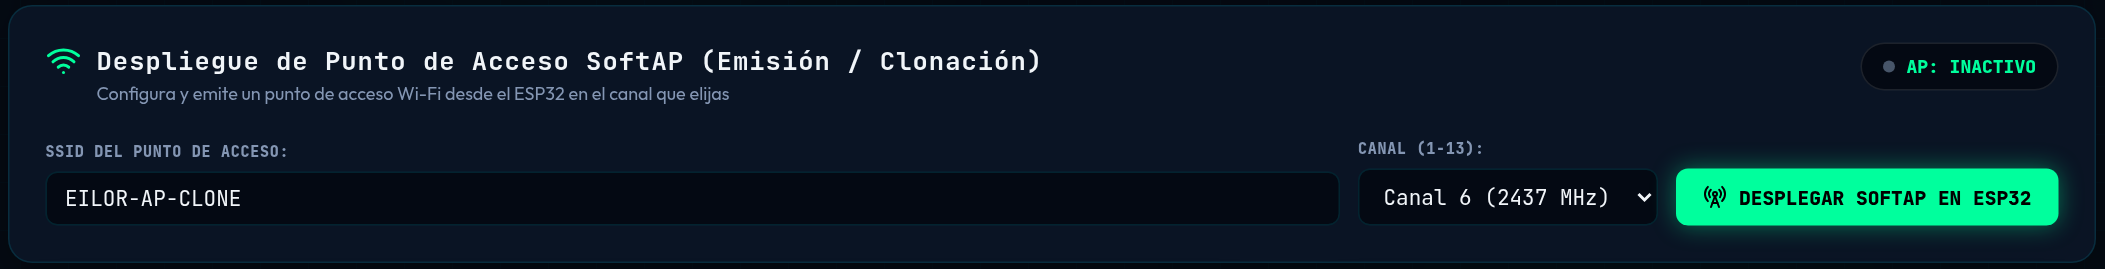
\includegraphics[width=0.98\linewidth]{figuras/cap-softap}}
\caption{Panel de despliegue del SoftAP: selección de SSID y canal del punto de acceso propio.}
\label{fig:softap}
\end{figure}

Cuando un invitado se conecta a la red emitida, su dispositivo es redirigido
automáticamente por el portal cautivo al formulario de registro
(Figura~\ref{fig:portal}), que solicita nombre, apellido y teléfono e incluye un
aviso explícito sobre la recolección de datos.

\begin{figure}[H]
\centering
\setlength{\fboxsep}{0pt}\setlength{\fboxrule}{0.4pt}%
\fcolorbox{gray!45}{white}{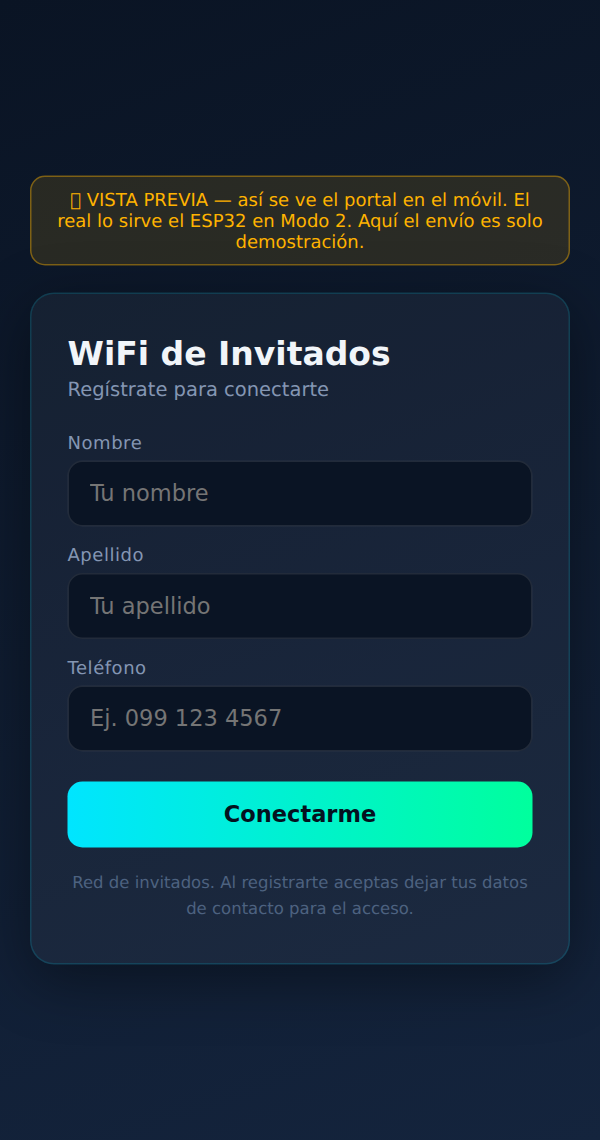
\includegraphics[height=8.5cm]{figuras/cap-portal}}
\caption{Formulario del portal cautivo tal como lo ve el invitado en su teléfono (vista previa).}
\label{fig:portal}
\end{figure}

\subsection{Análisis del espectro y radar BLE}
El núcleo analítico se visualiza en dos paneles contiguos
(Figura~\ref{fig:espectro-radar}): a la izquierda, el mapa de \emph{saturación
espectral} de los canales 1 al 13, con el canal más limpio, el más saturado y el
canal recomendado del conjunto no solapado 1/6/11; a la derecha, el \emph{radar de
proximidad BLE}, que ubica las balizas de forma radial según su RSSI. Ambos se
actualizan en vivo con cada ciclo de escaneo.

\begin{figure}[H]
\centering
\setlength{\fboxsep}{0pt}\setlength{\fboxrule}{0.4pt}%
\fcolorbox{gray!45}{white}{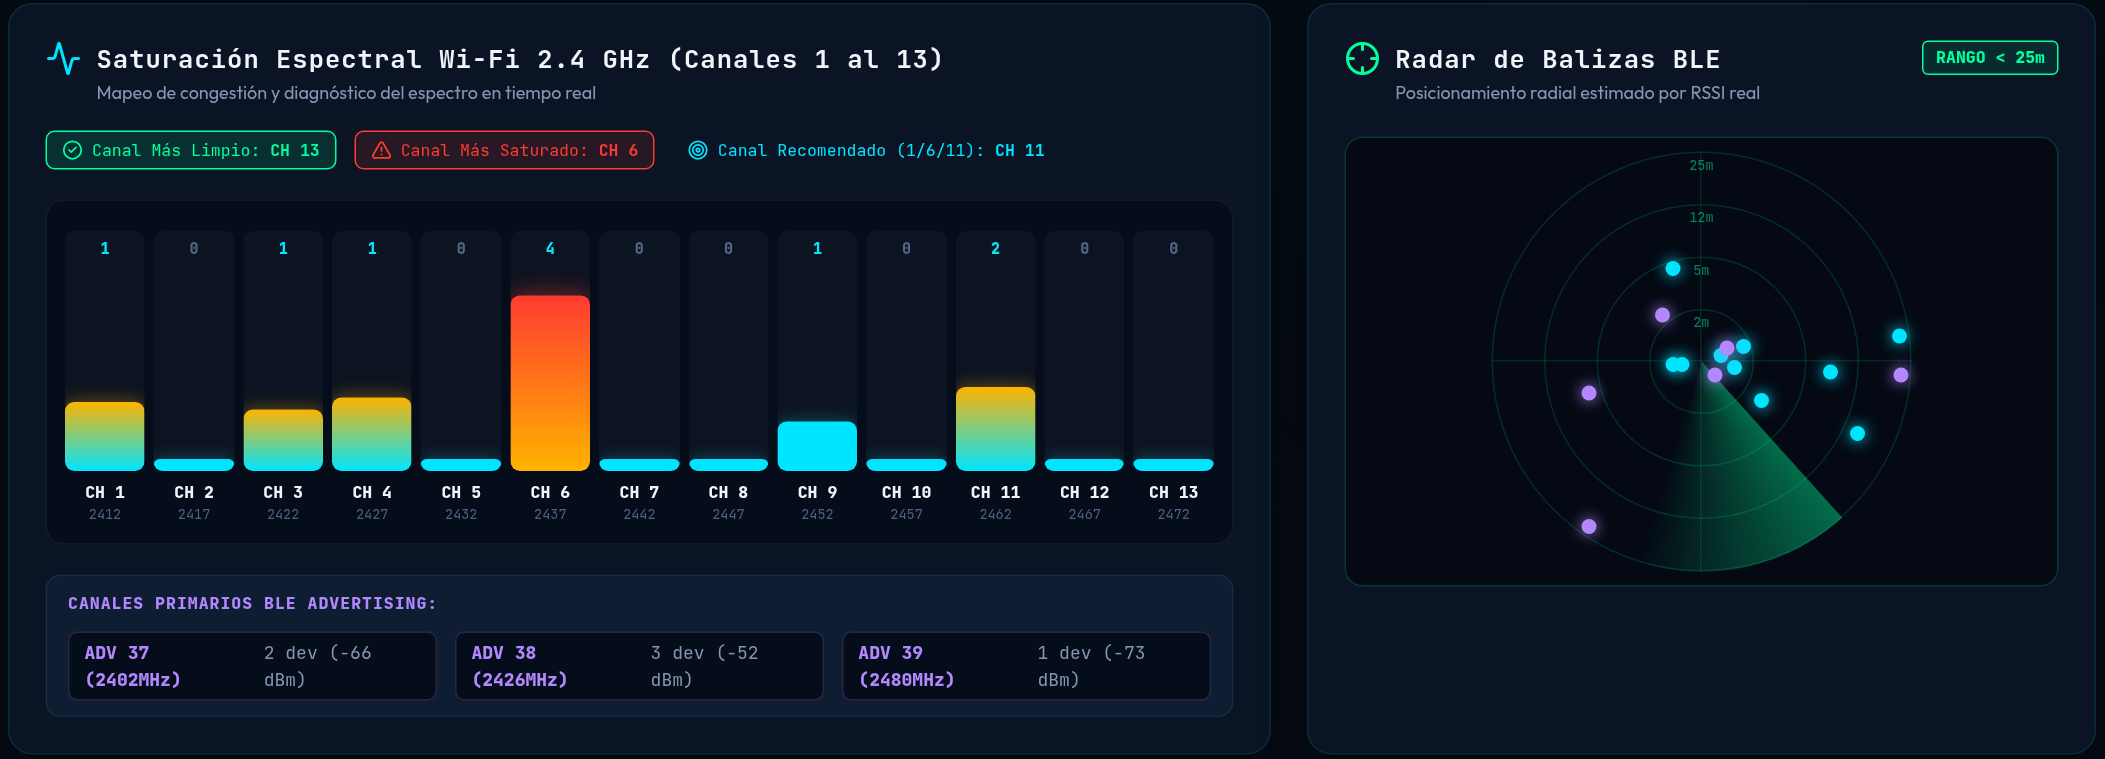
\includegraphics[width=0.98\linewidth]{figuras/cap-espectro-radar}}
\caption{Saturación espectral Wi\nobreakdash-Fi (canales 1--13) y radar de proximidad BLE en tiempo real.}
\label{fig:espectro-radar}
\end{figure}

\subsection{Telemetría y flujo de comandos}
El \emph{Panel de Telemetría} (Figura~\ref{fig:telemetria}) presenta una consola en
vivo con las tramas WebSocket, los eventos de conexión y las respuestas de comandos,
acompañada de una gráfica de serie temporal (dispositivos activos y paquetes por
minuto). Es la herramienta principal de diagnóstico del enlace en la demostración.

\begin{figure}[H]
\centering
\setlength{\fboxsep}{0pt}\setlength{\fboxrule}{0.4pt}%
\fcolorbox{gray!45}{white}{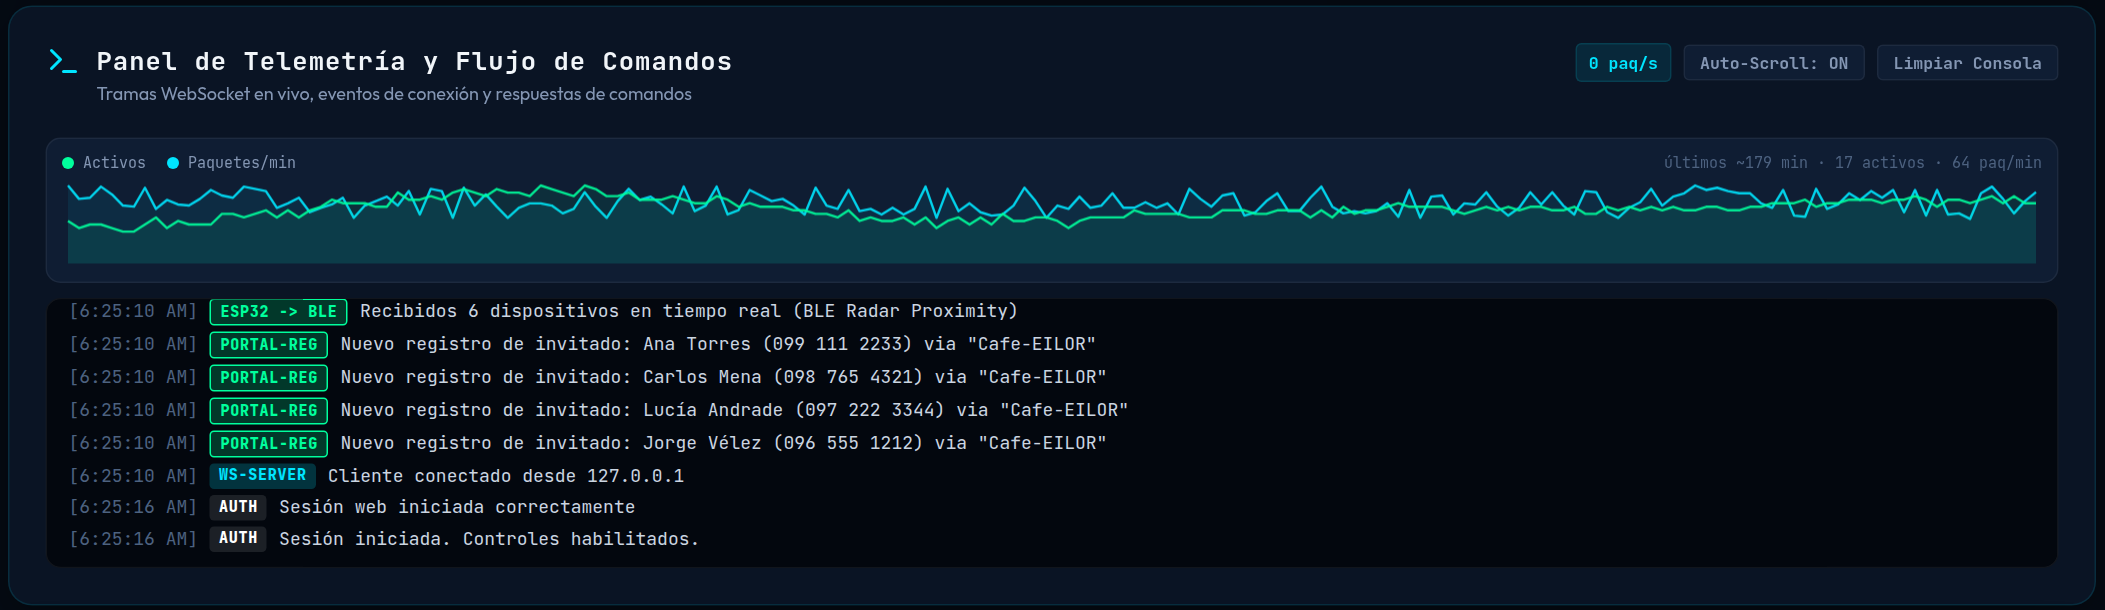
\includegraphics[width=0.98\linewidth]{figuras/cap-telemetria}}
\caption{Panel de telemetría: consola de tramas WebSocket y serie temporal de actividad.}
\label{fig:telemetria}
\end{figure}

\subsection{Inventario de dispositivos}
La tabla de \emph{Registro de Dispositivos} (Figura~\ref{fig:dispositivos})
enumera cada dispositivo detectado con su tipo, nombre/SSID, dirección MAC/BSSID,
fabricante (por OUI), canal, RSSI, distancia estimada y tipo de seguridad. Los
puntos de acceso sospechosos de \emph{gemelo malicioso} se marcan con una etiqueta
«Gemelo», y las direcciones aleatorizadas se rotulan como «MAC Aleatoria
(privacidad)». La tabla admite filtrado por tipo (Wi\nobreakdash-Fi/Bluetooth) y
búsqueda por SSID o MAC.

\begin{figure}[H]
\centering
\setlength{\fboxsep}{0pt}\setlength{\fboxrule}{0.4pt}%
\fcolorbox{gray!45}{white}{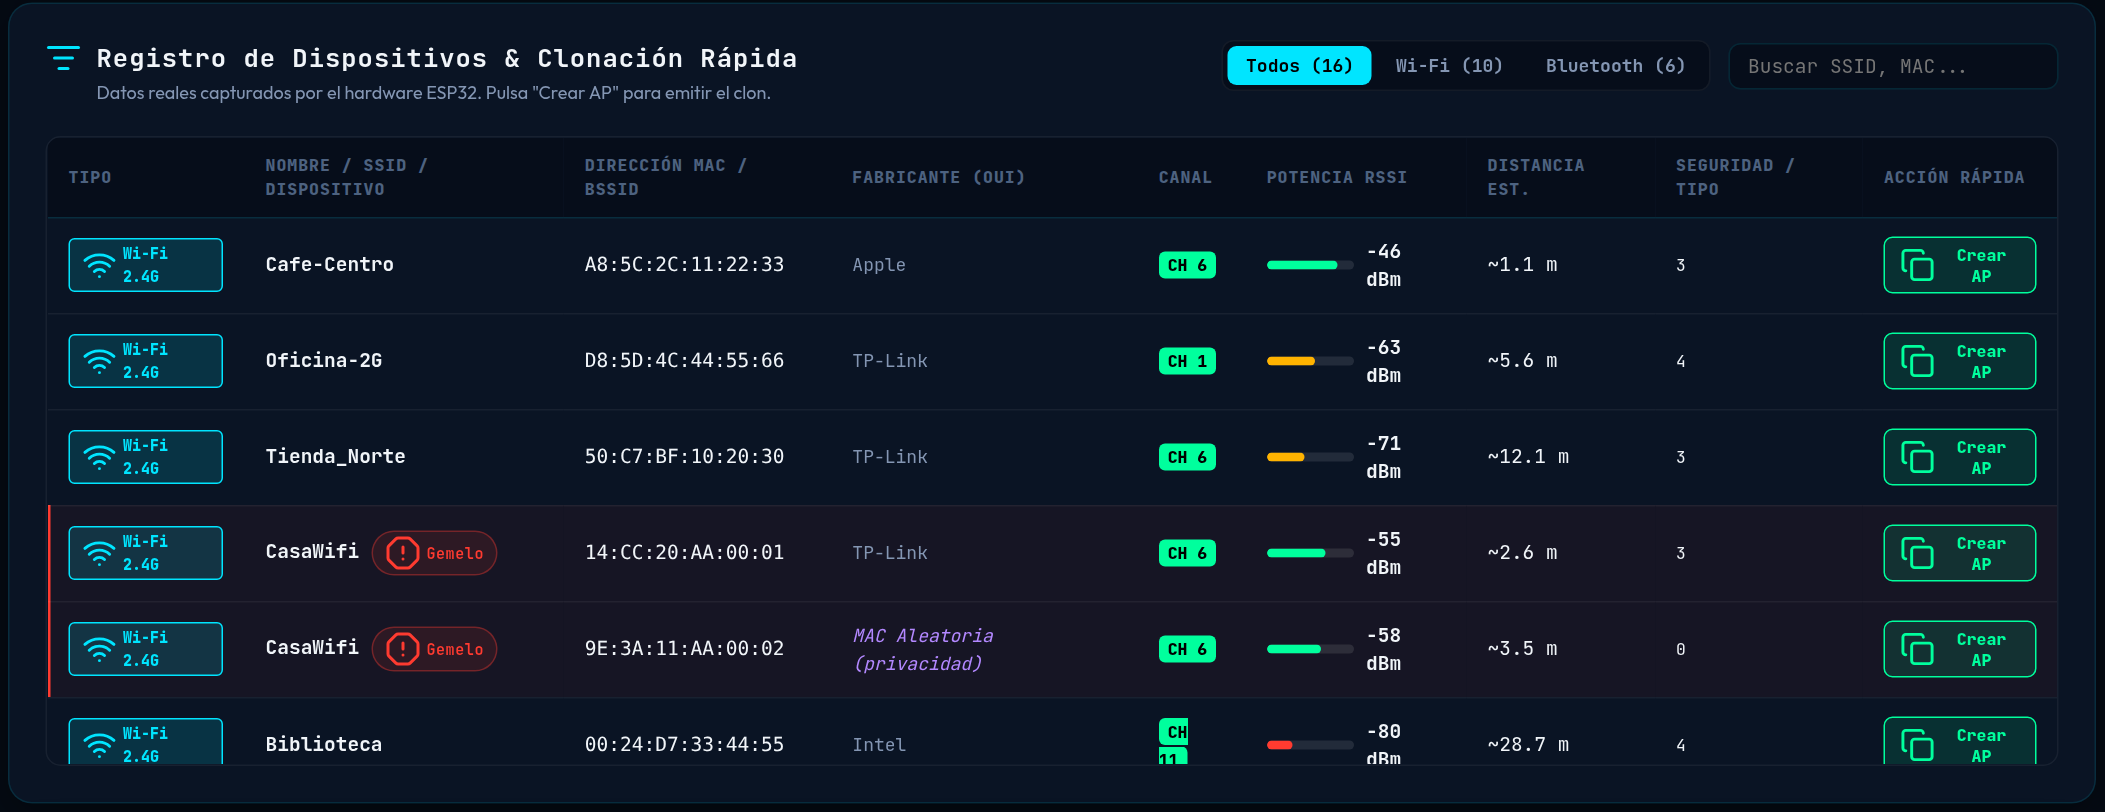
\includegraphics[width=0.98\linewidth]{figuras/cap-dispositivos}}
\caption{Inventario de dispositivos con fabricante por OUI, marcado de gemelo malicioso y de MAC aleatorizada.}
\label{fig:dispositivos}
\end{figure}

\subsection{Registros del portal cautivo}
La sección \emph{Registros del Portal Cautivo} (Figura~\ref{fig:registros-plat})
lista en tiempo real las altas de invitados (nombre, apellido, teléfono, red y
fecha). Desde allí se puede \emph{Exportar CSV} (con BOM UTF\nobreakdash-8 para su
apertura correcta en hojas de cálculo) o \emph{Borrar} los registros; ambas acciones
exigen sesión autenticada.

\begin{figure}[H]
\centering
\setlength{\fboxsep}{0pt}\setlength{\fboxrule}{0.4pt}%
\fcolorbox{gray!45}{white}{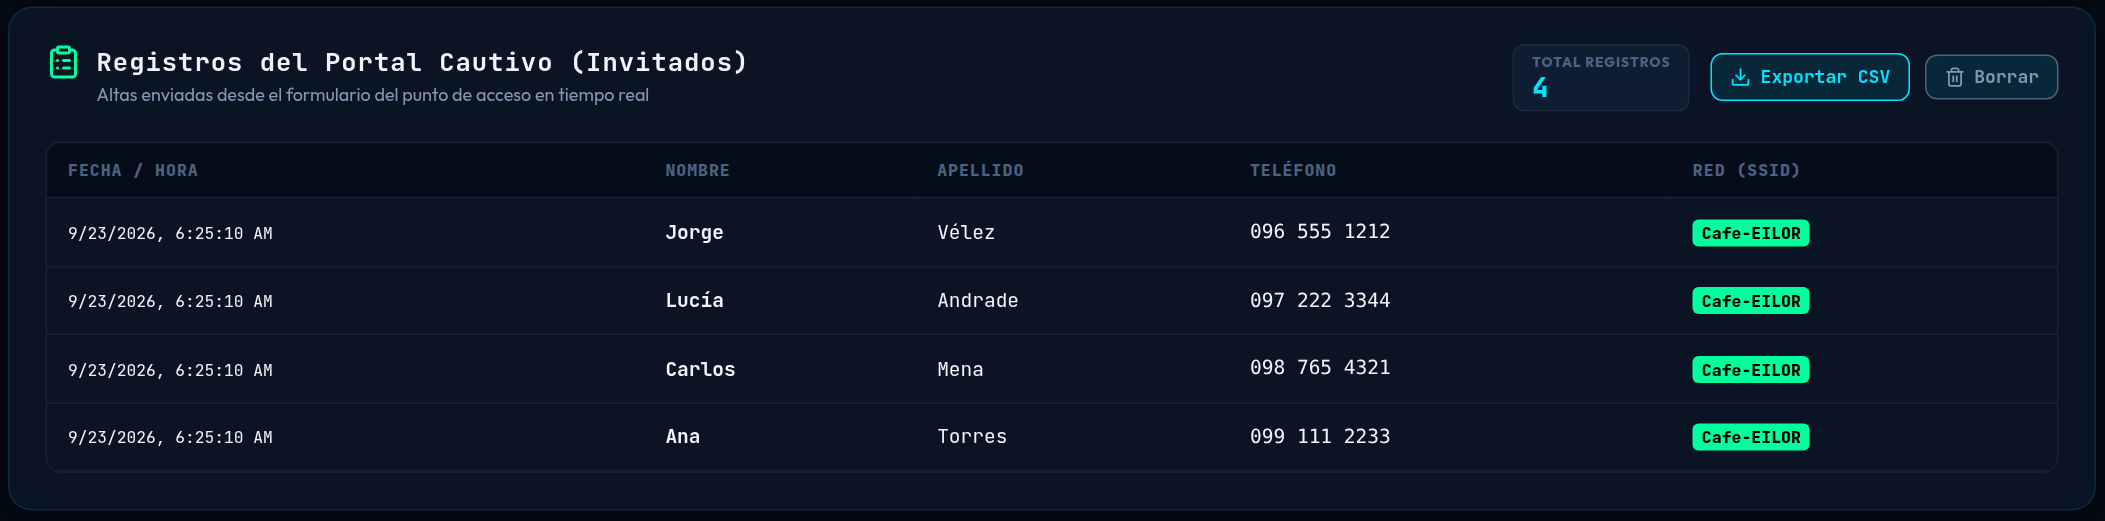
\includegraphics[width=0.98\linewidth]{figuras/cap-registros}}
\caption{Registros del portal cautivo en el \emph{dashboard}, con exportación restringida a la sesión.}
\label{fig:registros-plat}
\end{figure}

\section{Diseño de la interfaz web}
El frontend se construyó sin \emph{frameworks}, con HTML, CSS y JavaScript nativos,
priorizando la transparencia y la ligereza. El diseño visual adopta una estética de
«tablero táctico» oscuro, definida mediante \emph{variables CSS} (tokens de color y
tipografía) que unifican la apariencia. La Tabla~\ref{tab:frontend} resume las
decisiones de diseño y los archivos que las materializan.

\begin{table}[H]
\centering
\caption{Composición del frontend de la plataforma}
\label{tab:frontend}
\footnotesize
\begin{tabularx}{\linewidth}{@{}l l X@{}}
\toprule
\textbf{Aspecto} & \textbf{Archivo} & \textbf{Descripción} \\
\midrule
Estructura & \code{public/index.html} & Secciones del \emph{dashboard} y superposición de \emph{login} (419 líneas) \\
Lógica & \code{public/app.js} & Cliente WebSocket, renderizadores y control de sesión (913 líneas) \\
Estilos & \code{public/styles.css} & Tokens de color, tipografía y componentes «tácticos» (1\,272 líneas) \\
Portal & \code{public/portal-preview.html} & Vista previa del formulario del portal cautivo \\
Tipografía & Google Fonts & \emph{Outfit} (display) y \emph{JetBrains Mono} (monoespaciada) \\
Iconografía & Lucide & Iconos vectoriales ligeros vía CDN \\
\bottomrule
\end{tabularx}
\end{table}

El cliente mantiene un objeto de estado en memoria (\code{state}) que consolida los
dispositivos, el mapa de calor, la serie temporal y los registros; ante cada evento
WebSocket se actualiza el estado y se invoca únicamente al renderizador afectado
(mapa de calor, radar, tabla, registros o serie temporal), evitando redibujar toda
la página. El token de sesión se guarda en \code{localStorage} para no repetir el
inicio de sesión entre recargas.

\section{Comunicación entre la web, el servidor y el ESP32}
La plataforma se comunica con el dispositivo de forma \emph{indirecta}: nunca habla
directamente con el ESP32, sino a través del servidor Node.js, que actúa como
concentrador. Existen dos canales complementarios:

\begin{itemize}[leftmargin=1.4em]
  \item \textbf{WebSocket (tiempo real):} tanto el ESP32 como los navegadores
  mantienen una conexión WebSocket persistente con el servidor. El ESP32 envía sus
  escaneos, \emph{heartbeats} y registros de invitados; el servidor los procesa y
  \emph{difunde} (\emph{push}) los resultados a todos los navegadores conectados. En
  sentido inverso, los comandos de la web (cambio de modo, despliegue de SoftAP)
  viajan al servidor, que los reenvía al ESP32 por el mismo canal.
  \item \textbf{API REST (consultas y control):} la web dispone además de catorce
  \emph{endpoints} HTTP (Tabla~\ref{tab:rest}) para inicio de sesión, consultas de
  estado, control y gestión de registros, empleados en las operaciones que no
  requieren tiempo real.
\end{itemize}

La Figura~\ref{fig:comunicacion} ilustra el flujo de un comando de control emitido
desde la web hasta el ESP32 y la difusión de vuelta del nuevo estado.

\begin{figure}[H]
\centering
\begin{tikzpicture}[
  font=\small,
  n/.style={rectangle,rounded corners=3pt,draw,thick,align=center,minimum height=1.0cm,minimum width=2.7cm},
  arr/.style={-{Latex[length=2.4mm]},thick},
  lbl/.style={font=\scriptsize\itshape,align=center}
]
\node[n,fill=gray!8] (web) {Navegador\\(dashboard)};
\node[n,fill=eiloremerald!12,right=3.2cm of web] (srv) {Servidor Node.js\\(concentrador)};
\node[n,fill=eilorcyan!10,right=3.2cm of srv] (esp) {ESP32\\(firmware)};

\draw[arr] ([yshift=6pt]web.east) -- node[lbl,above]{1. comando\\(set\_mode + token)} ([yshift=6pt]srv.west);
\draw[arr] ([yshift=6pt]srv.east) -- node[lbl,above]{2. reenvío\\WSS} ([yshift=6pt]esp.west);
\draw[arr] ([yshift=-6pt]esp.west) -- node[lbl,below]{3. escaneo /\\heartbeat} ([yshift=-6pt]srv.east);
\draw[arr] ([yshift=-6pt]srv.west) -- node[lbl,below]{4. push\\scan\_update} ([yshift=-6pt]web.east);
\end{tikzpicture}
\caption{Flujo de comunicación web $\leftrightarrow$ servidor $\leftrightarrow$ ESP32 (el servidor concentra ambos sentidos).}
\label{fig:comunicacion}
\end{figure}

Las acciones de control validan el \emph{token de sesión} antes de reenviarse al
dispositivo; un comando WebSocket sin token válido recibe un evento
\code{auth\_error} y no se ejecuta. La ingesta de escaneos, a su vez, puede
restringirse con un \emph{token de dispositivo} opcional
(\code{EILOR\_DEVICE\_TOKEN}). El detalle de los mensajes WebSocket y de los
\emph{endpoints} REST se encuentra en la Sección~\ref{cap:diseno} del diseño
detallado, y la publicación segura del servicio mediante el túnel de Cloudflare, en
el Capítulo~\ref{cap:cloudflare}.

\section{Vista pública en producción}
La Figura~\ref{fig:produccion} muestra la plataforma tal como se sirve en el dominio
público \plataformaurl{} sobre HTTPS/WSS, evidenciando el despliegue real de extremo
a extremo (dispositivo, túnel, servidor y cliente).

\begin{figure}[H]
\centering
\setlength{\fboxsep}{0pt}\setlength{\fboxrule}{0.4pt}%
\fcolorbox{gray!45}{white}{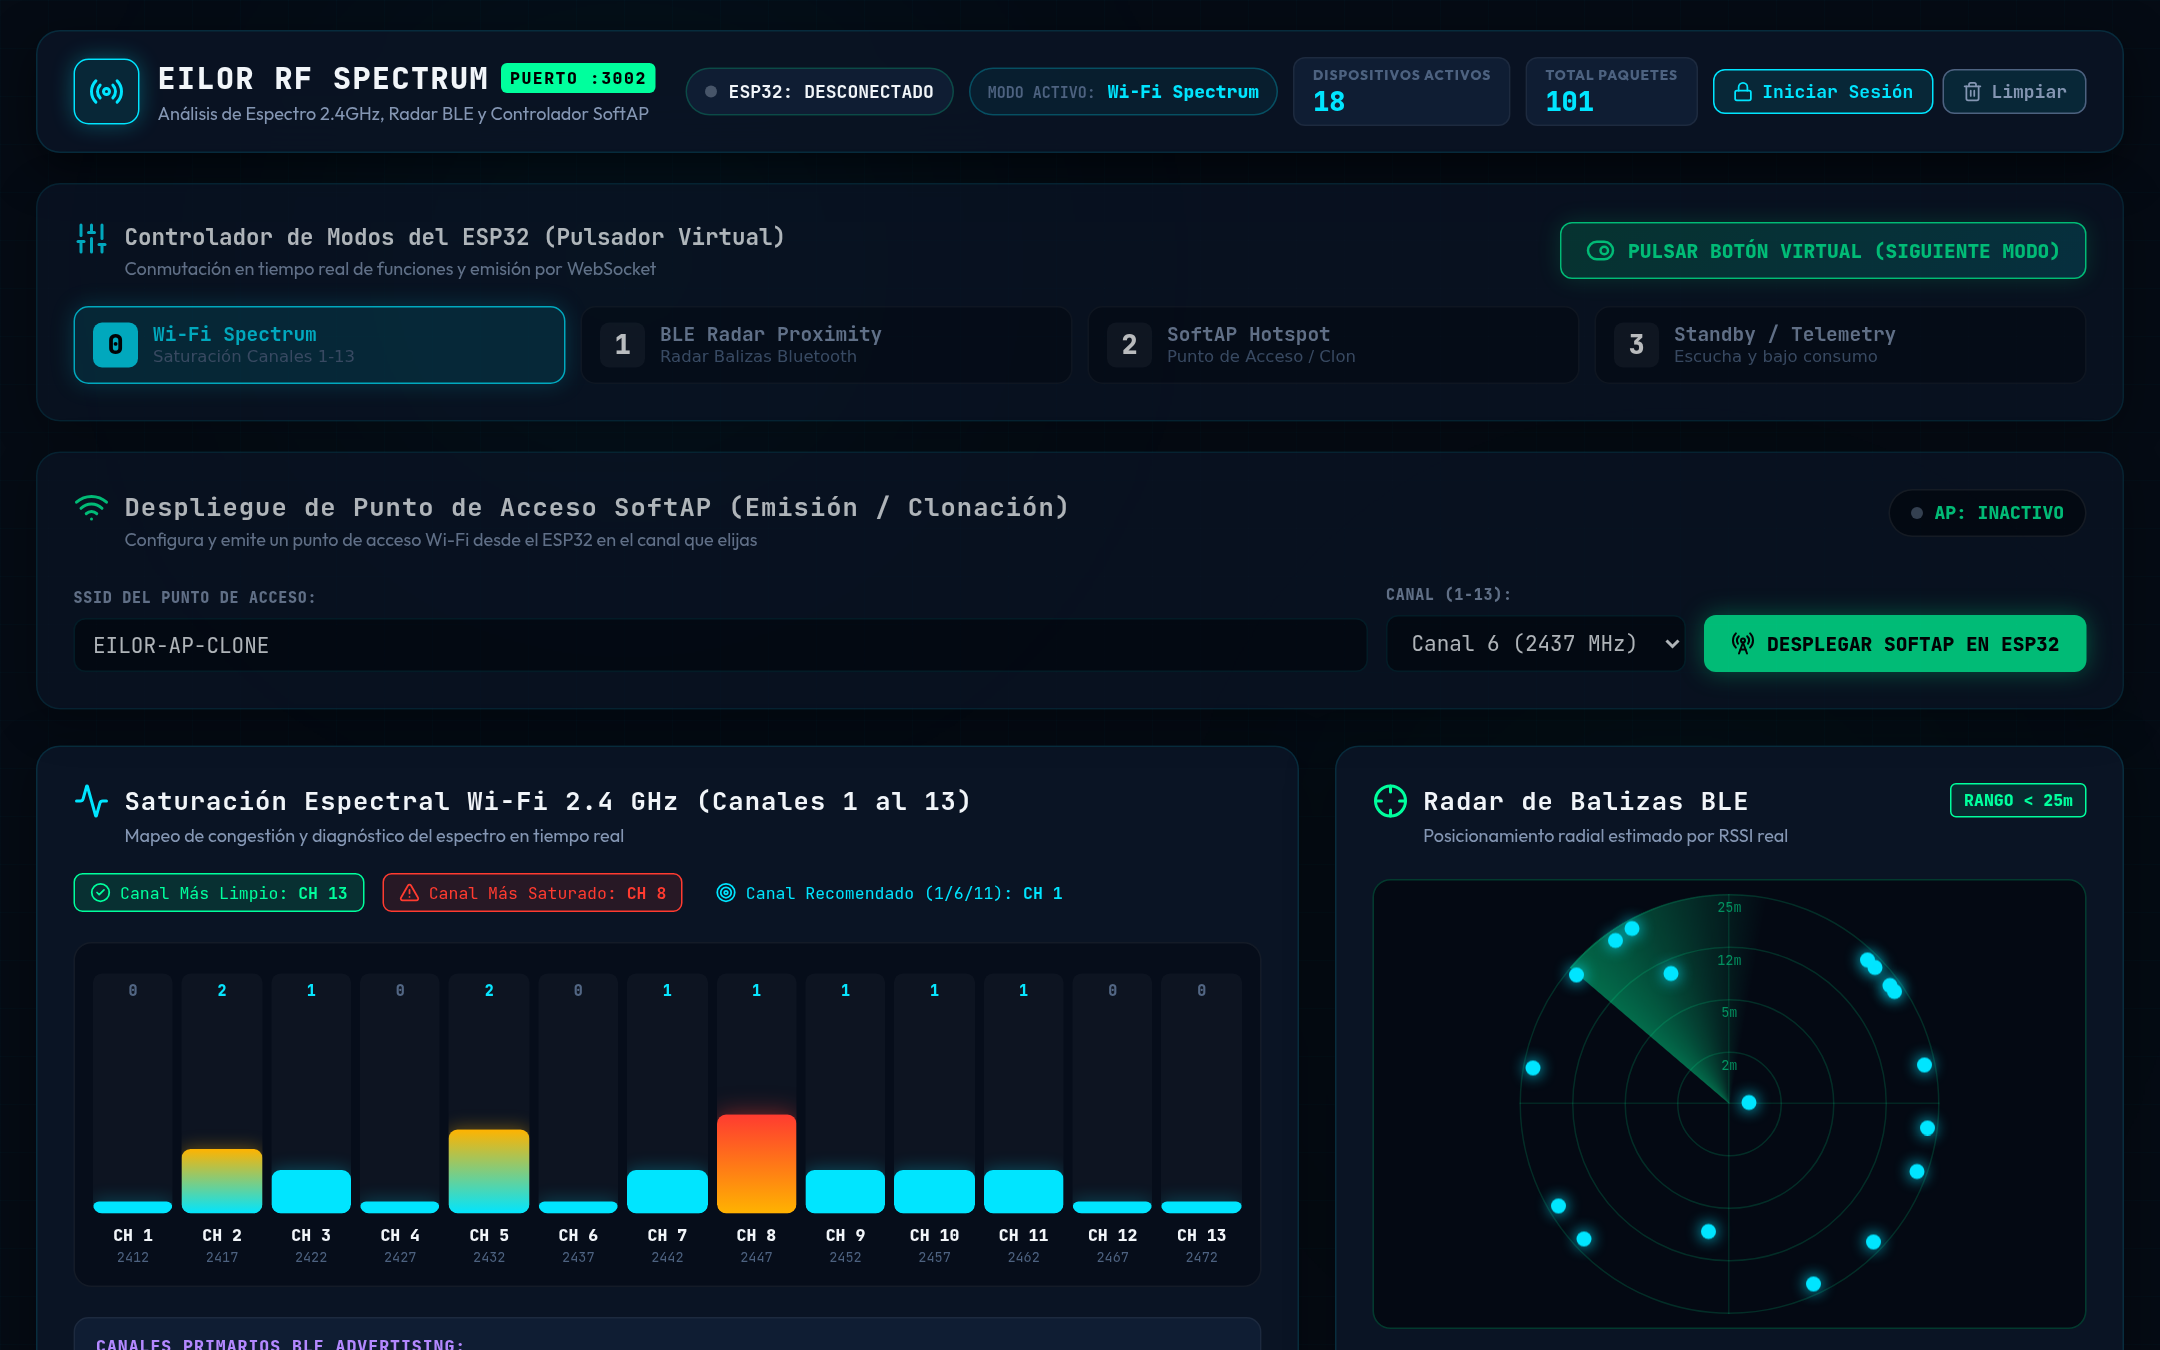
\includegraphics[width=0.98\linewidth]{figuras/cap-produccion}}
\caption{Plataforma EILOR publicada en \code{esp.orellanadigitalco.trade} a través del túnel de Cloudflare.}
\label{fig:produccion}
\end{figure}
